\section{ХОД РАБОТЫ}

\subsection{Текст задания}

Для всех вариантов необходимо выполнить следующее: 

\begin{itemize}

  \item определить типы и функции в соответствии со своим вариантом задания;
  \item в функции main() реализовать демонстрацию работы созданных функций.

\end{itemize}

Необходимо определить структуру Complex для хранения комплексных чисел и ряд функций для работы с ними. Пример заголовочного файла complex.h представлен на рисунке~\ref{lst:task}. 

\begin{lstlisting}[caption=Пример описания структуры Complex и объявления функций,label=lst:task]
  struct Complex
  {
    double re;
    double im;
  };

  Complex Add(Complex c1, Complex c2);
  Complex Sub(Complex c1, Complex c2);
  Complex Mul(Complex c1, Complex c2);
  Complex Div(Complex c1, Complex c2);
  
  void PrintComplex(Complex c);
\end{lstlisting}

Все функции должны возвращать новое комплексное число, содержащее результат операции.

\subsection{Особенности разработанной программы}

В ходе проведения данной лабораторной работы была разработана программа для выполнения арифметических операций над комплексными числами, представляющая пользователю простой в использовании консольный интерфейс, защищённый от ошибок некорректного ввода.

Главное меню программы, изображенное на рисунке~\ref{fig:menu}, состоит из трёх частей. Первая часть отвечает за выводит на экран комплексных чисел, с которыми в данный момент времени работает пользователь. Вторая часть предоставляет возможность изменить комплексные числа. Третья часть главного меню позволяет пользователю выбрать требуемую арифметическую операцию. 

\begin{figure}[htbp]
  \centering
  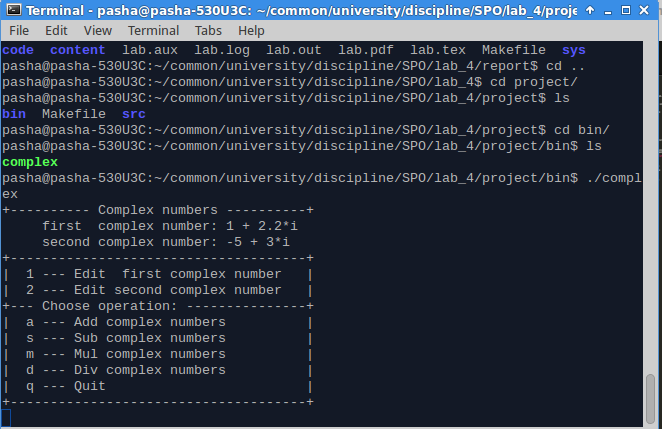
\includegraphics[width=150mm,height=92mm]{img/menu}
  \caption{Главное меню программы}\label{fig:menu}
\end{figure}

После того, как пользователь выбрал необходимую операцию программа производит вычисления. Полученное в результате вычислений новое комплексное число представляется пользователю в алгебраической и показательной формах. Пример корректной работы программы проиллюстрирован на рисунке~\ref{fig:correct}.

\pagebreak
\begin{figure}[h!]
  \centering
  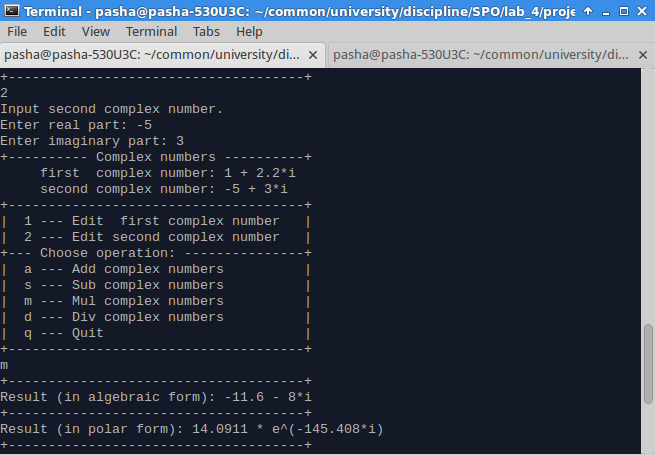
\includegraphics[width=150mm,height=92mm]{img/correct}
  \caption{Пример корректной работы программы}\label{fig:correct}
\end{figure}

Если выполнение какой-либо операции невозможно, то на экран выводится сообщение об ошибке. Пример вывода сообщения об ошибке на экран при попытке деления на нулевое комплексное число продемонстрирован на рисунке~\ref{fig:error}.

\begin{figure}[h!]
  \centering
  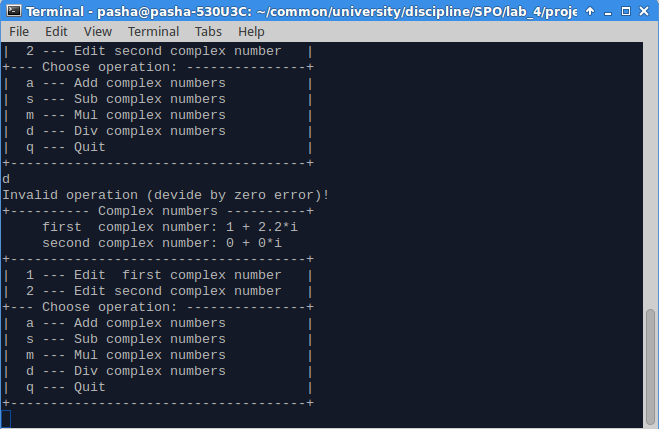
\includegraphics[width=150mm,height=92mm]{img/error}
  \caption{Пример вывода сообщения об ошибке}\label{fig:error}
\end{figure}

Исходный текст разработанной программы расположен в приложении~А.

\newpage